\pdfminorversion=4
\documentclass[aspectratio=169]{beamer}

\mode<presentation>
{
  \usetheme{default}
  \usecolortheme{default}
  \usefonttheme{default}
  \setbeamertemplate{navigation symbols}{}
  \setbeamertemplate{caption}[numbered]
  \setbeamertemplate{footline}[frame number]  % or "page number"
  \setbeamercolor{frametitle}{fg=white}
  \setbeamercolor{footline}{fg=black}
} 

\usepackage[english]{babel}
\usepackage{inputenc}
\usepackage{tikz}
\usepackage{courier}
\usepackage{array}
\usepackage{bold-extra}
\usepackage{minted}
\usepackage[thicklines]{cancel}
\usepackage{fancyvrb}

\xdefinecolor{dianablue}{rgb}{0.18,0.24,0.31}
\xdefinecolor{darkblue}{rgb}{0.1,0.1,0.7}
\xdefinecolor{darkgreen}{rgb}{0,0.5,0}
\xdefinecolor{darkgrey}{rgb}{0.35,0.35,0.35}
\xdefinecolor{darkorange}{rgb}{0.8,0.5,0}
\xdefinecolor{darkred}{rgb}{0.7,0,0}
\definecolor{darkgreen}{rgb}{0,0.6,0}
\definecolor{mauve}{rgb}{0.58,0,0.82}

\title[2024-10-19-preCHEP-2024-hsf-training]{Analysis of HSF-Training event data}
\author{Jim Pivarski}
\institute{Princeton University -- IRIS-HEP}
\date{October 19, 2024}

\usetikzlibrary{shapes.callouts}

\begin{document}

\logo{\pgfputat{\pgfxy(0.11, 7.4)}{\pgfbox[right,base]{\tikz{\filldraw[fill=dianablue, draw=none] (0 cm, 0 cm) rectangle (50 cm, 1 cm);}\mbox{\hspace{-8 cm}
\includegraphics[height=1 cm]{princeton-logo-long.png}\hspace{0.1 cm}\raisebox{0.1 cm}{
\includegraphics[height=0.8 cm]{iris-hep-logo-long.png}}\hspace{0.1 cm}}}}}

\begin{frame}
  \titlepage
\end{frame}

\logo{\pgfputat{\pgfxy(0.11, 7.4)}{\pgfbox[right,base]{\tikz{\filldraw[fill=dianablue, draw=none] (0 cm, 0 cm) rectangle (50 cm, 1 cm);}\mbox{\hspace{-8 cm}
\includegraphics[height=1 cm]{princeton-logo.png}\hspace{0.1 cm}\raisebox{0.1 cm}{
\includegraphics[height=0.8 cm]{iris-hep-logo.png}}\hspace{0.1 cm}}}}}

% Uncomment these lines for an automatically generated outline.
%\begin{frame}{Outline}
%  \tableofcontents
%\end{frame}

% START START START START START START START START START START START START START

\begin{frame}{Why are we analyzing student data?}
\Large
\vspace{0.5 cm}
At the IRIS-HEP Retreat, we realized that the frequency of training events and our milestones are not data-driven, but we now have a significant dataset and can change that.
\end{frame}

\begin{frame}{Sources of data}
\Large
\vspace{0.5 cm}
\begin{itemize}\setlength{\itemsep}{0.35 cm}
\item<1-> Indico registrations: 24 events since 2019
\item<2-> Pre- and post-event surveys: students are required to fill these out (Zoom password is at the end of the pre-event survey), \\ 17 events since 2021

\vspace{0.25 cm}
\uncover<3->{Surveys have been analyzed before, but not across all events.}

\item<4-> Website traffic: anonymized, but can identify unique visitors {\it each day}, since May 2023
\item<5-> Zoom and Slack activity for the February 2024 ``Analysis Pipelines'' event (at least)
\end{itemize}
\end{frame}

\begin{frame}{(Indico) Where do the registrants come from?}
\large
\vspace{0.5 cm}
\begin{center}
\only<1>{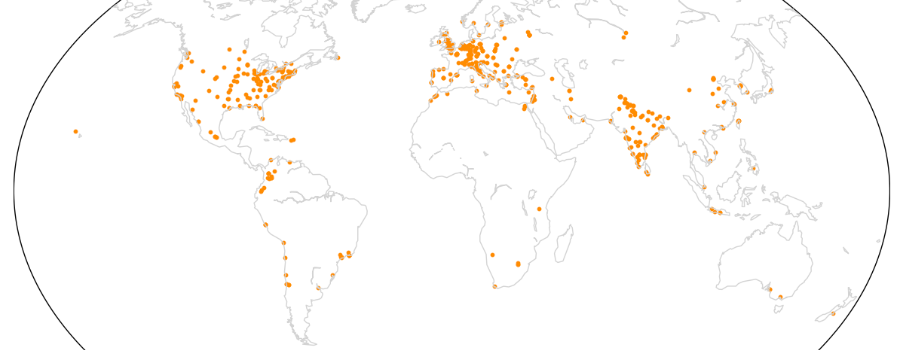
\includegraphics[width=\linewidth]{PLOTS/indico-registrations-map.png}\vspace{0.5 cm}}\only<2>{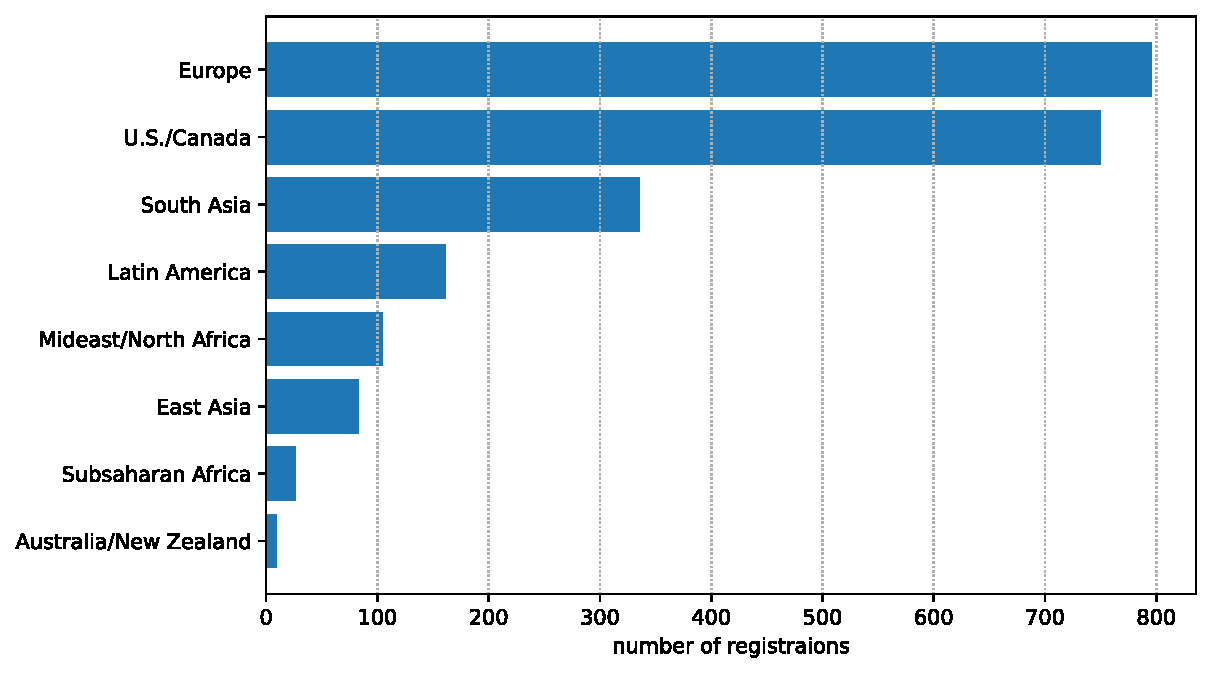
\includegraphics[width=0.8\linewidth]{PLOTS/indico-registrations-by-country.pdf}}

\vspace{0.35 cm}
\textcolor{gray}{(Note: only a fraction of the students who register actually attend.)}
\end{center}
\end{frame}

\begin{frame}{(Surveys) What kinds of students are these?}
\vspace{0.3 cm}
\begin{center}
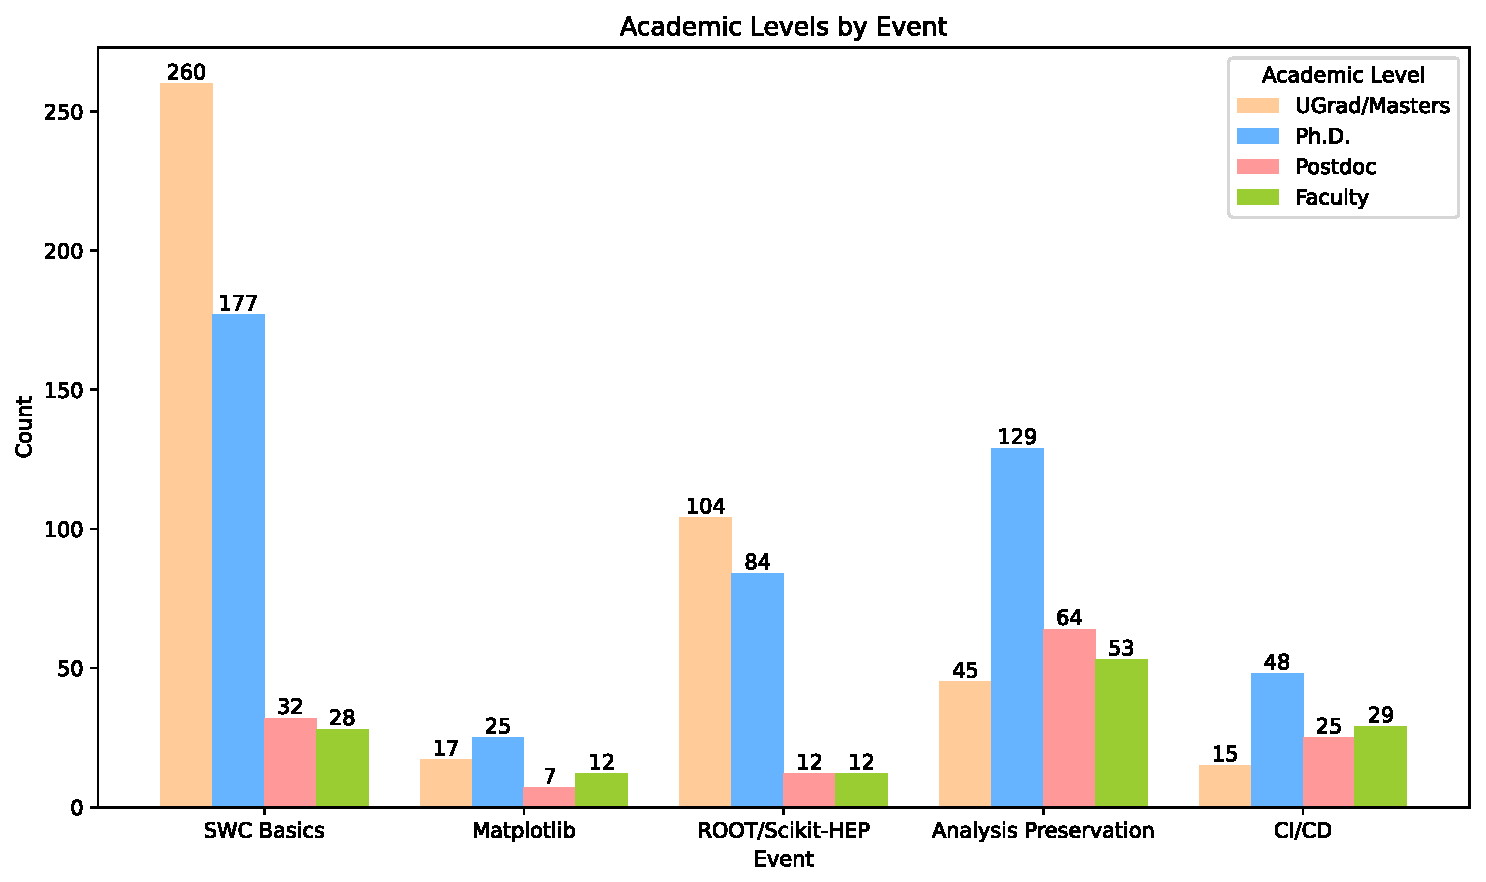
\includegraphics[width=0.9\linewidth]{PLOTS/academic-level-by-event.pdf}
\end{center}
\end{frame}

\begin{frame}{(Website) Who visits the website?}
\vspace{0.2 cm}
\begin{center}
\only<1>{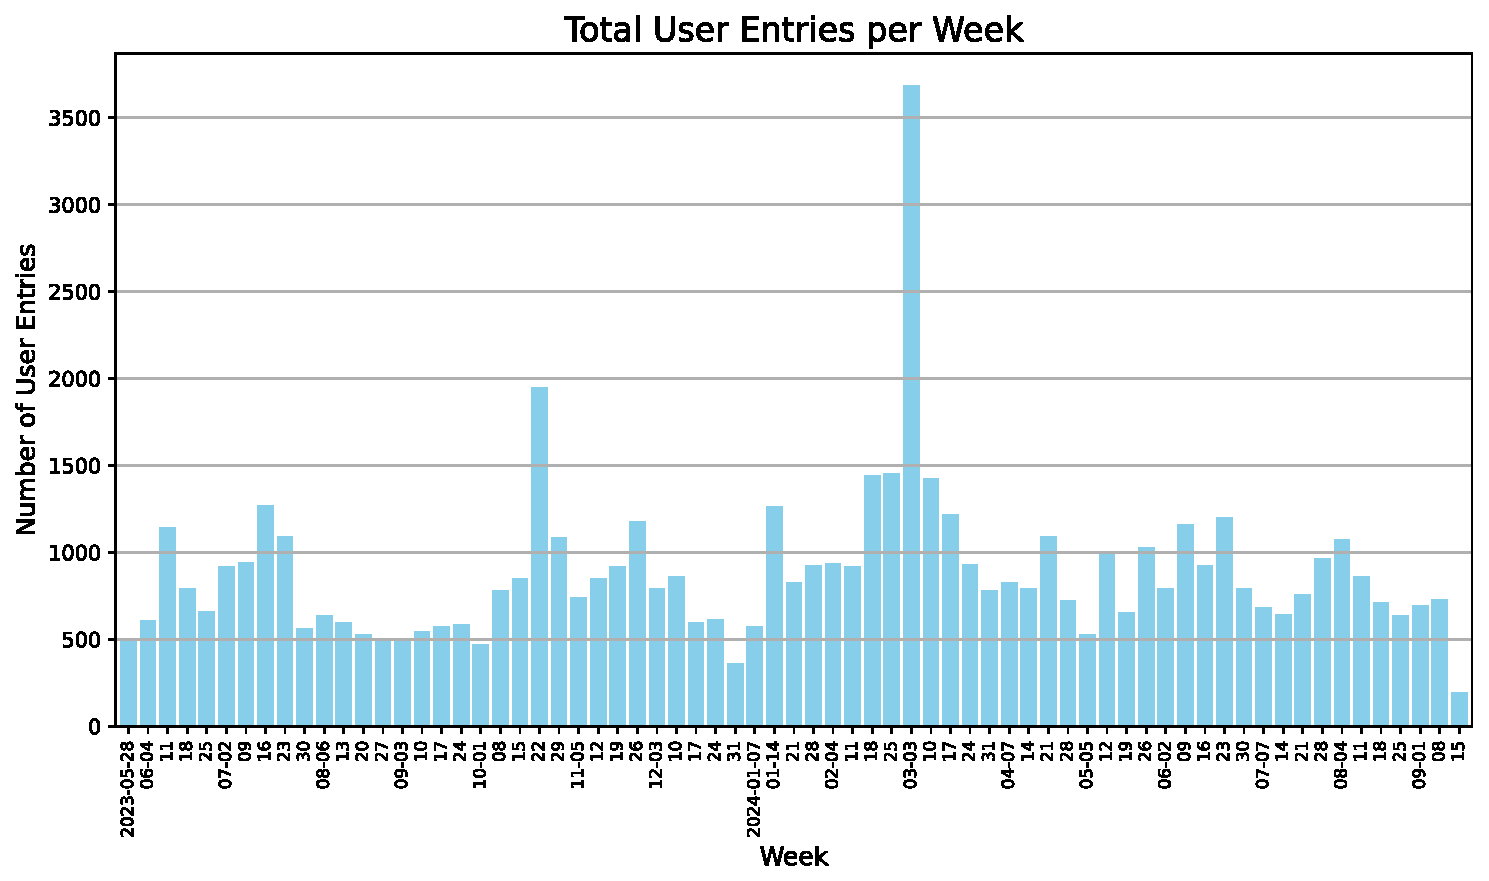
\includegraphics[width=0.93\linewidth]{PLOTS/website-access-per-week.pdf}}\only<2>{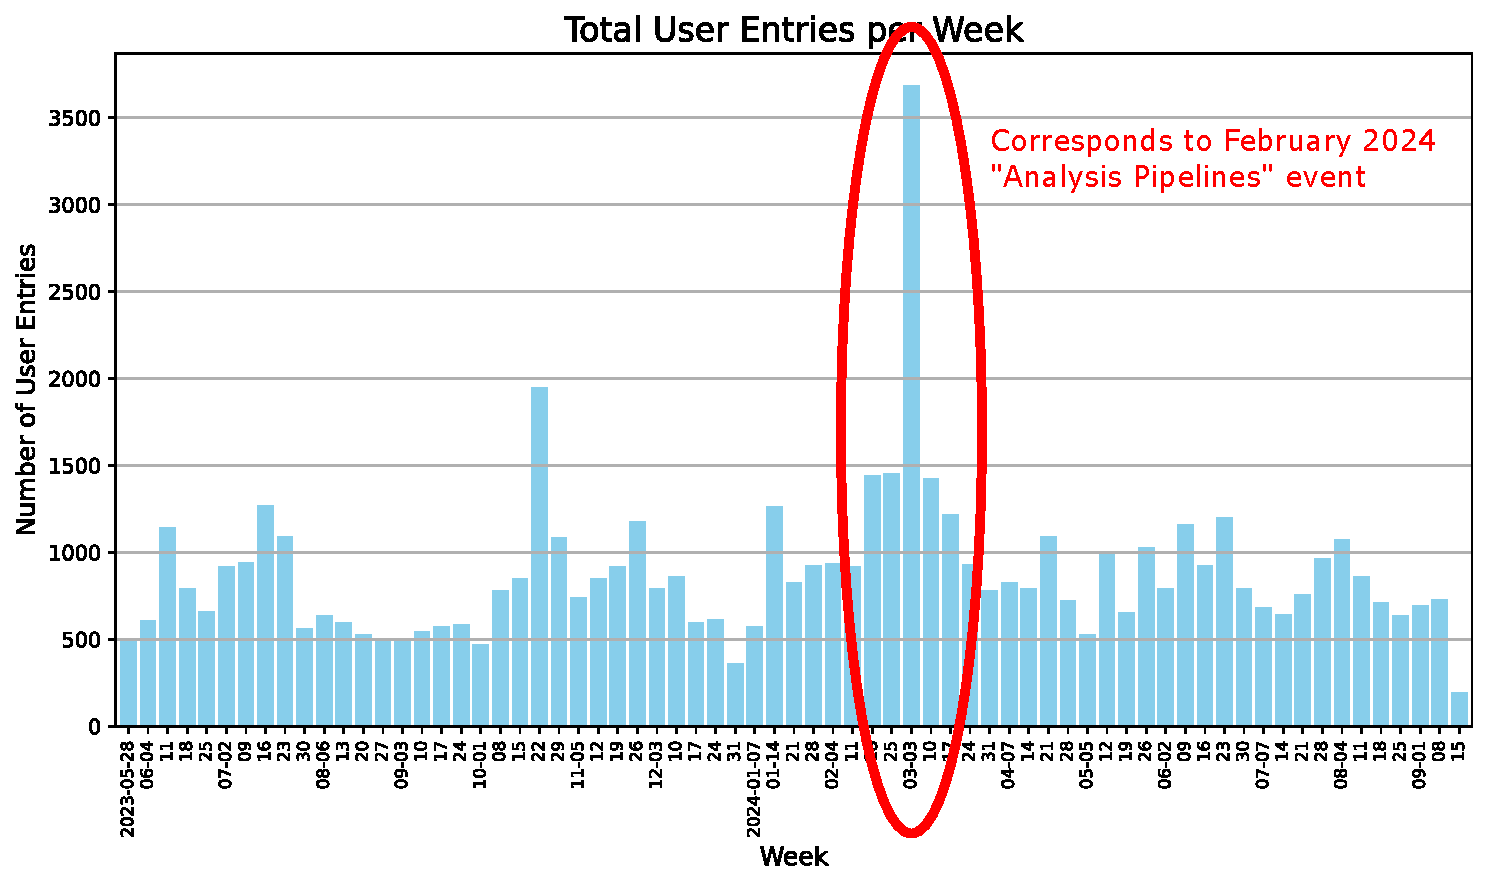
\includegraphics[width=0.93\linewidth]{PLOTS/website-access-per-week-2.pdf}}\only<3>{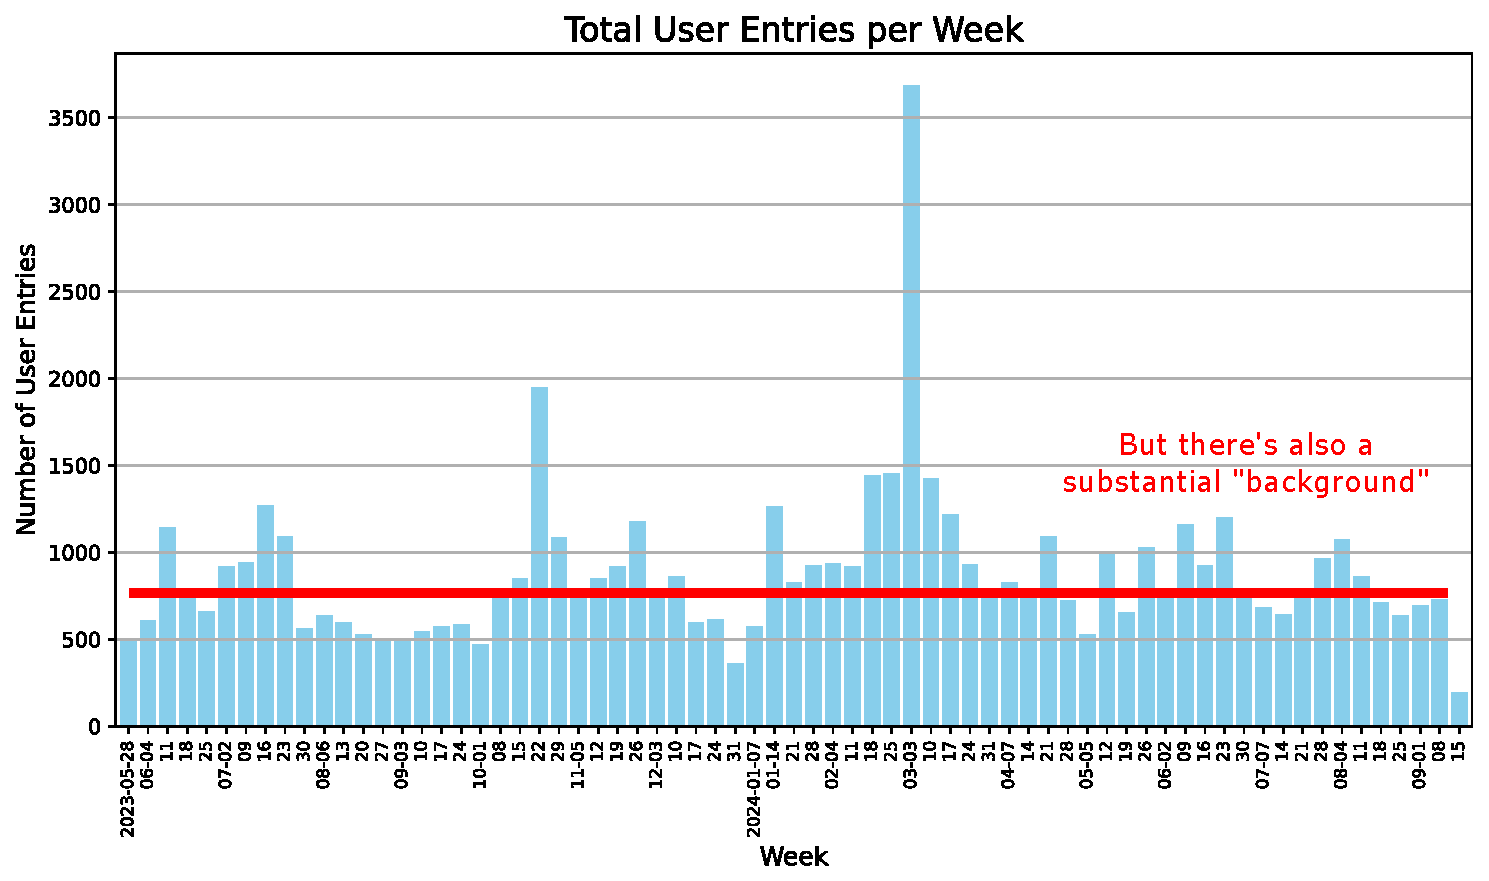
\includegraphics[width=0.93\linewidth]{PLOTS/website-access-per-week-3.pdf}}
\end{center}
\end{frame}

\begin{frame}{(Website) Are they studying the material or brief glance?}
\vspace{0.2 cm}
\begin{columns}
\column{1.1\linewidth}
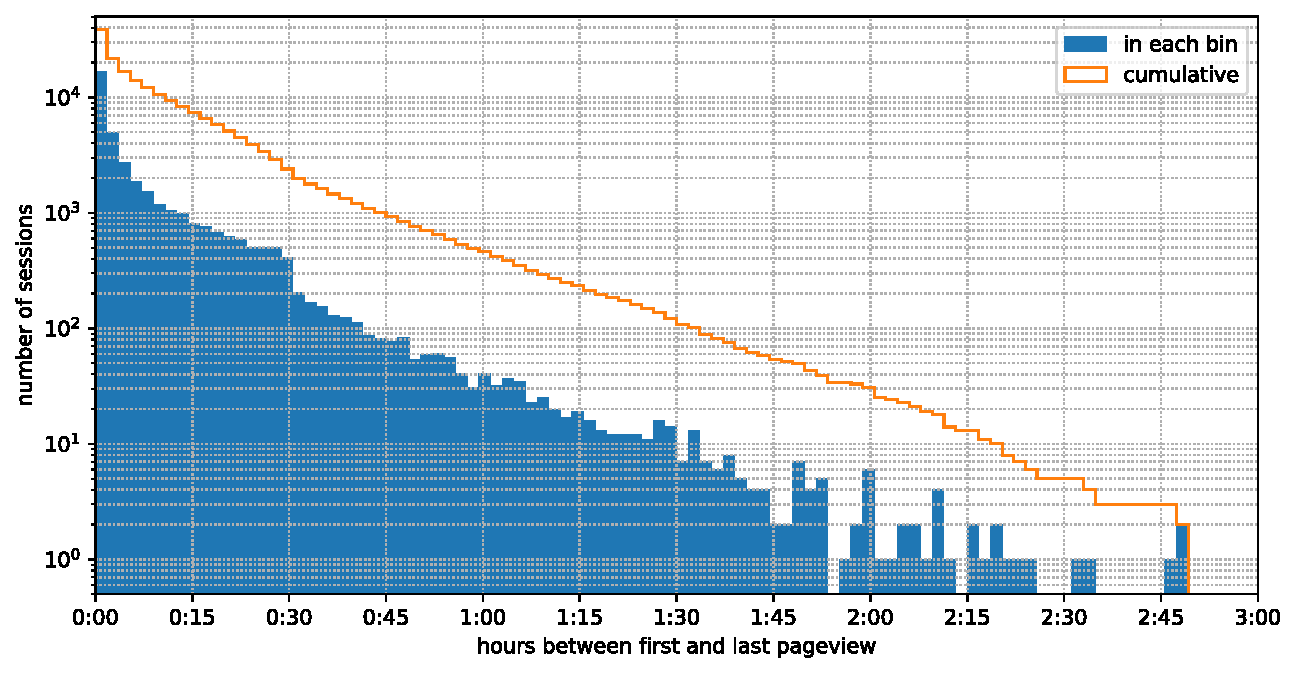
\includegraphics[width=\linewidth]{PLOTS/hours-per-session.pdf}
\end{columns}
\end{frame}

\begin{frame}{(Website) What are the most popular modules?}
\vspace{0.2 cm}
\begin{center}
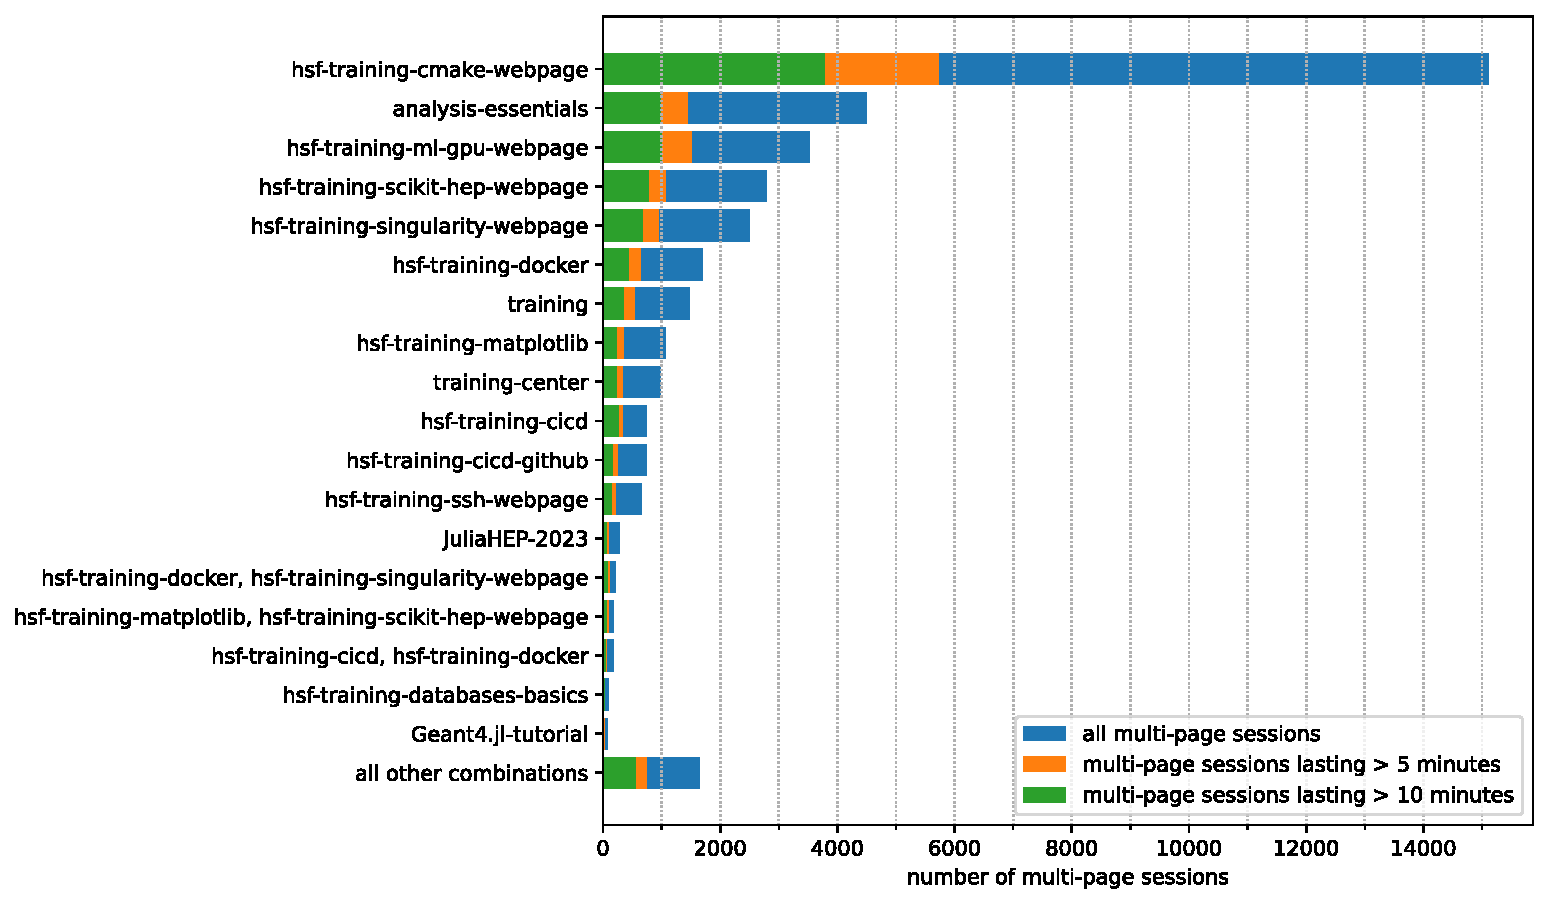
\includegraphics[width=0.95\linewidth]{PLOTS/most-popular-modules.pdf}
\end{center}
\end{frame}

\begin{frame}{(Website) Long-term website visits broken down by module}
\Large
\vspace{0.5 cm}
\begin{columns}
\column{1.1\linewidth}
\only<1>{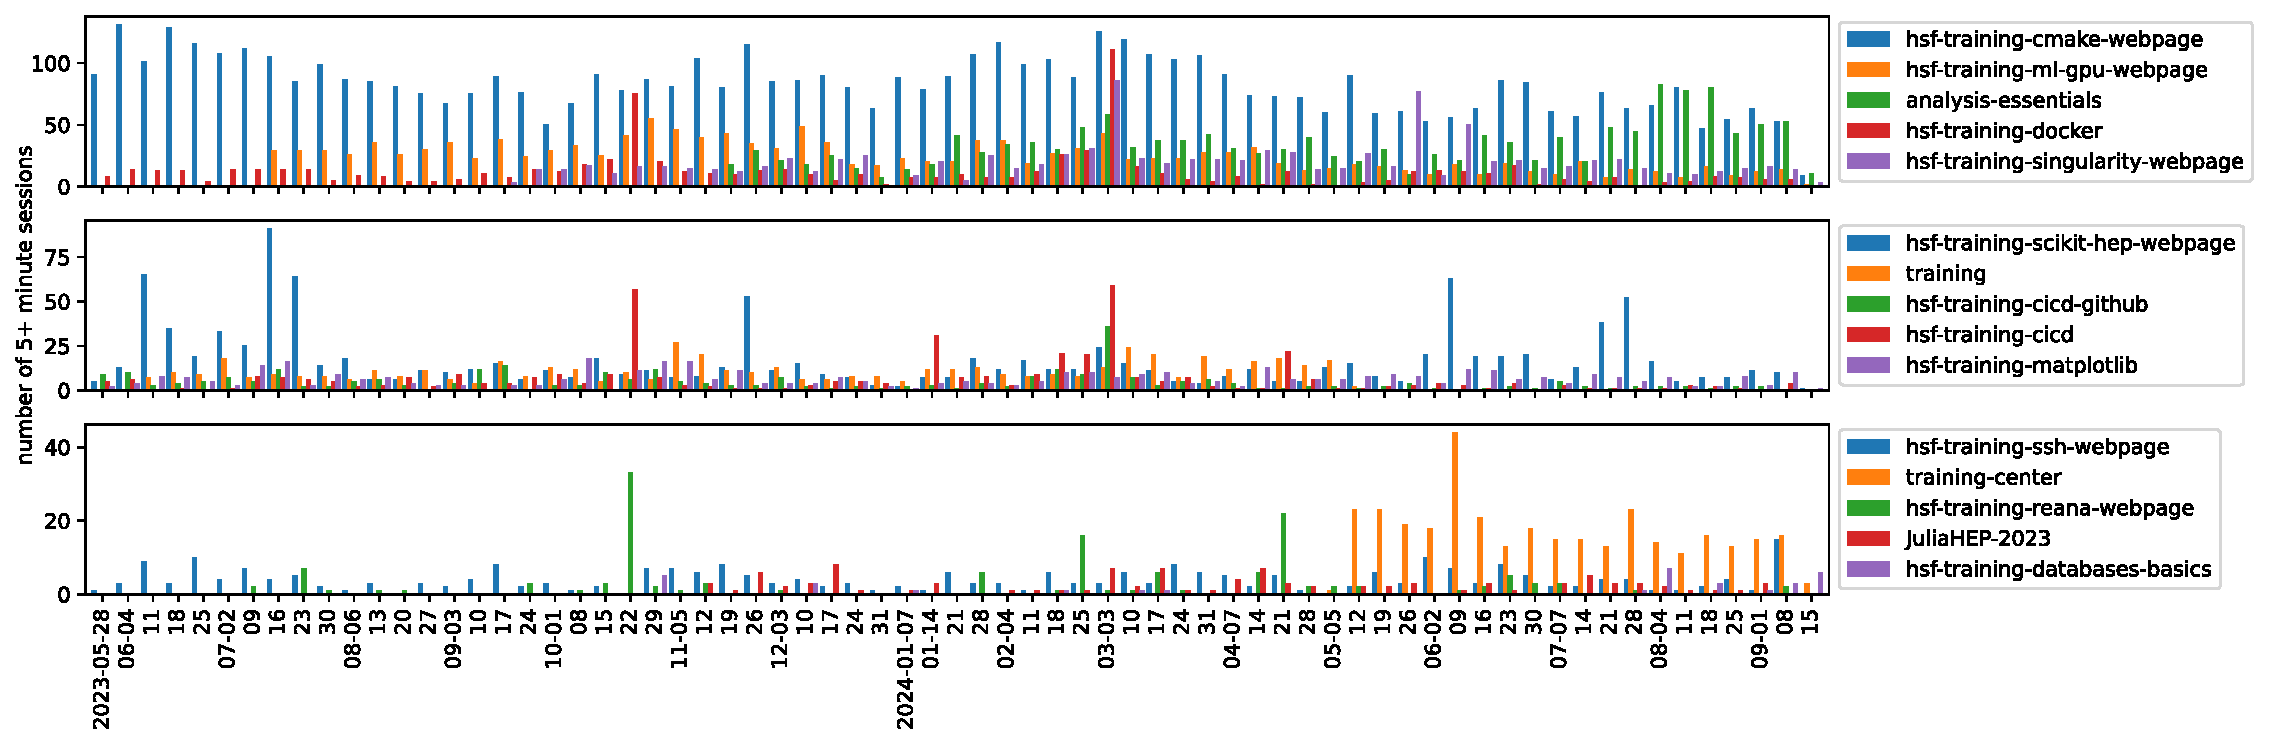
\includegraphics[width=\linewidth]{PLOTS/modules-accessed-per-week.pdf}}\only<2>{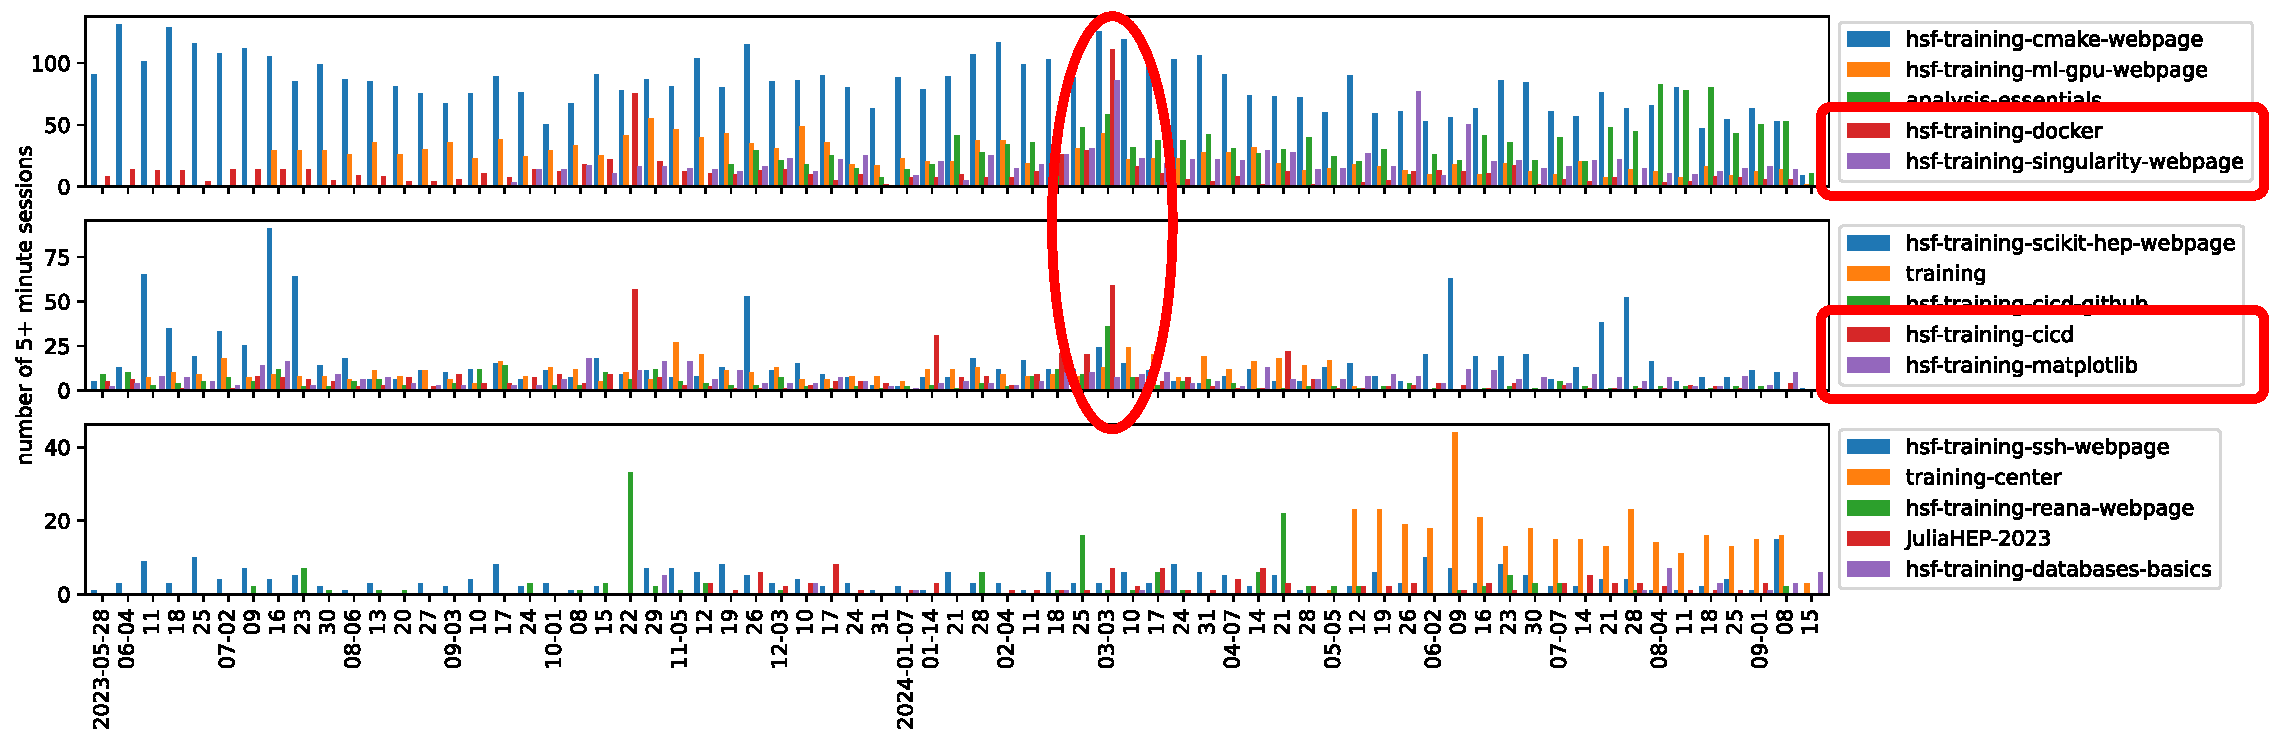
\includegraphics[width=\linewidth]{PLOTS/modules-accessed-per-week-2.pdf}}
\end{columns}

\vspace{0.5 cm}
\uncover<2>{This is the same training event we saw before. Let's zoom into it.}
\end{frame}

\begin{frame}{(Website) Modules in the training event, that week + 3 more weeks}
\Large
\vspace{0.5 cm}
\begin{columns}
\column{1.1\linewidth}
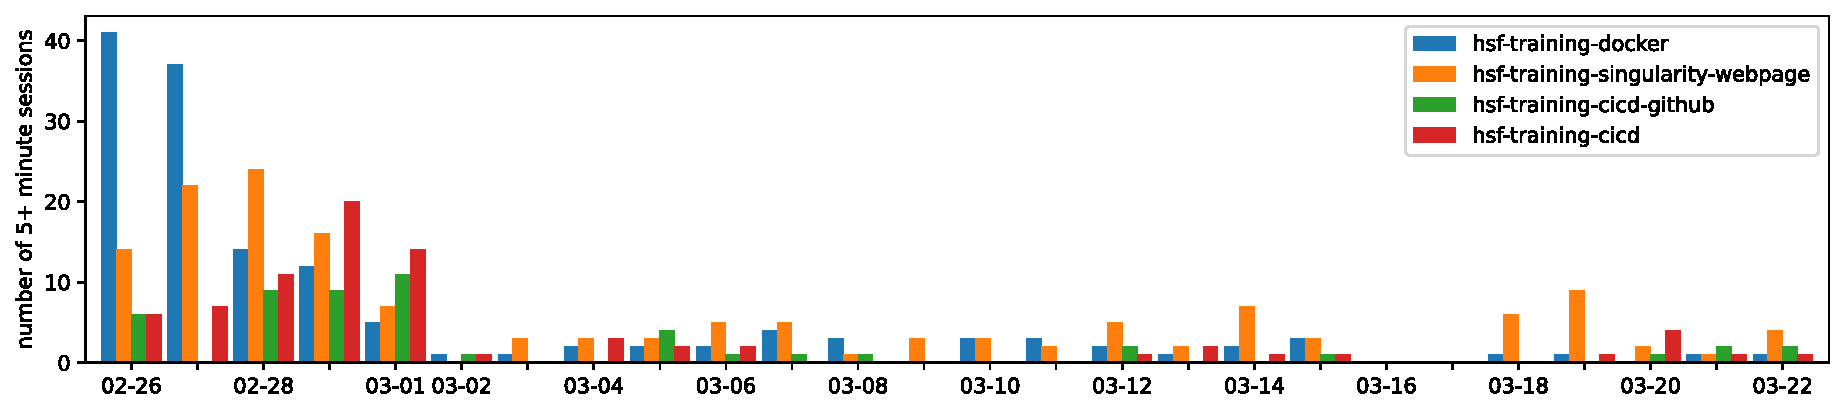
\includegraphics[width=\linewidth]{PLOTS/excess-during-pipelines-training.pdf}
\end{columns}

\vspace{1 cm}
\uncover<2>{We can do a sideband subtraction: ``excess'' visitors during the event minus (properly scaled) data from after the event.}
\end{frame}

\begin{frame}{(Website) Properties of the visitors, with sideband subtraction}
\Large
\vspace{0.5 cm}
\begin{columns}
\column{0.35\linewidth}
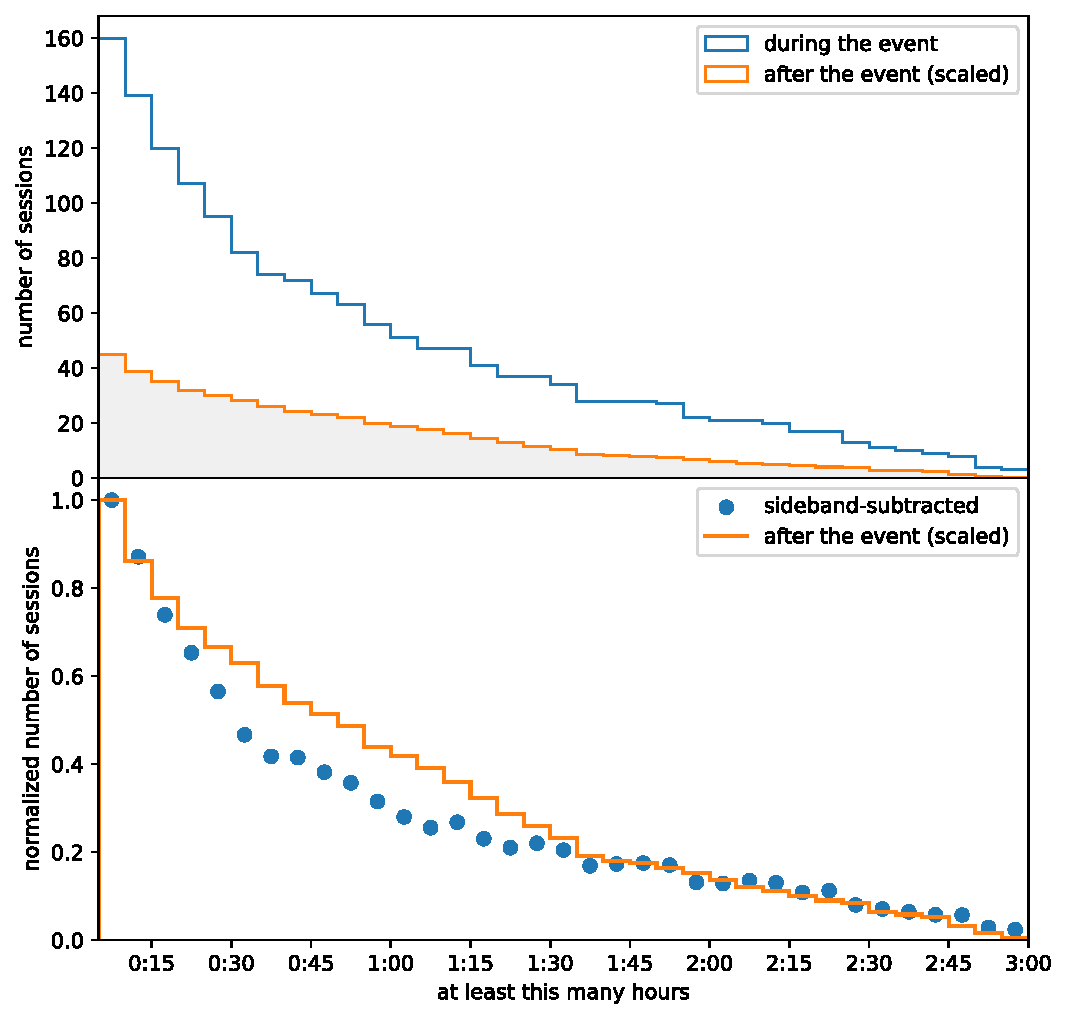
\includegraphics[width=\linewidth]{PLOTS/during-and-after-event-time-spent.pdf}

\column{0.35\linewidth}
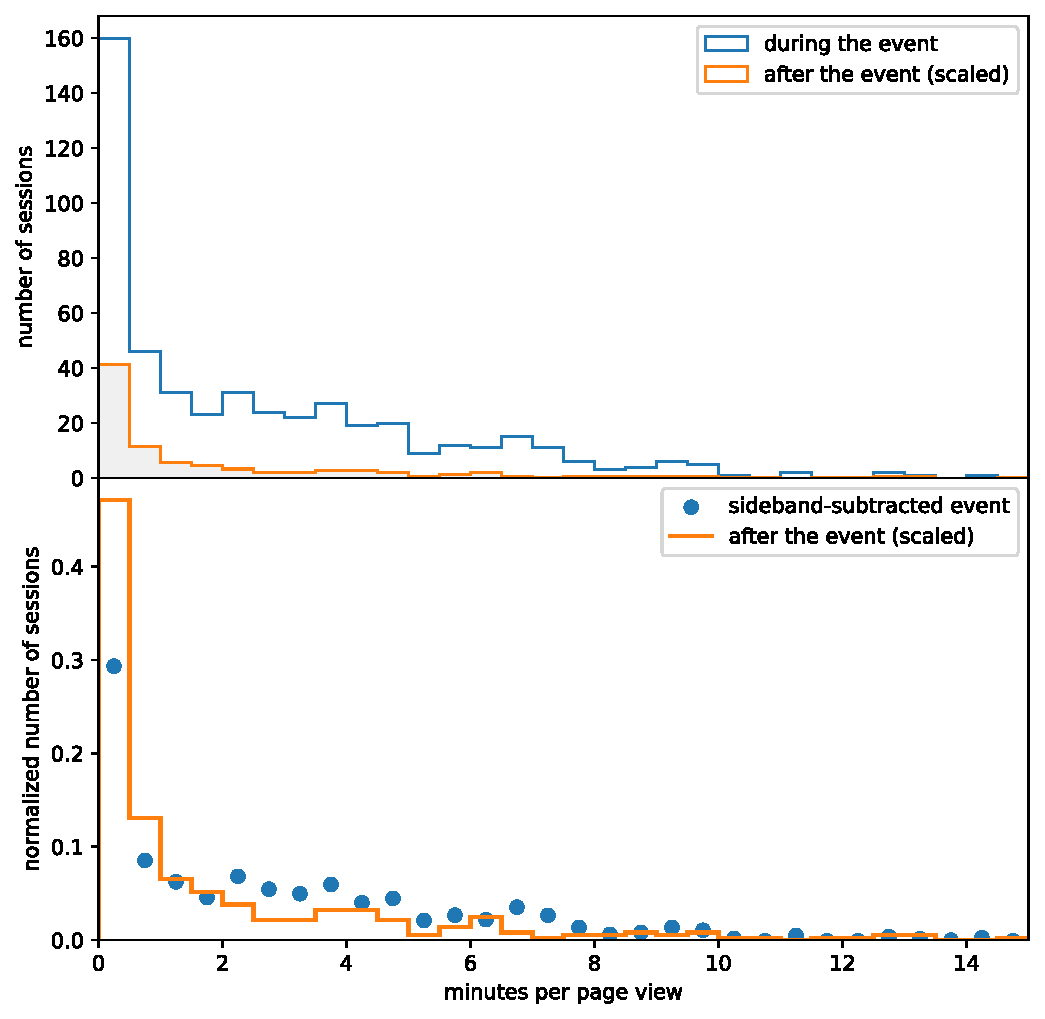
\includegraphics[width=\linewidth]{PLOTS/during-and-after-event-time-per-page-view.pdf}

\column{0.35\linewidth}
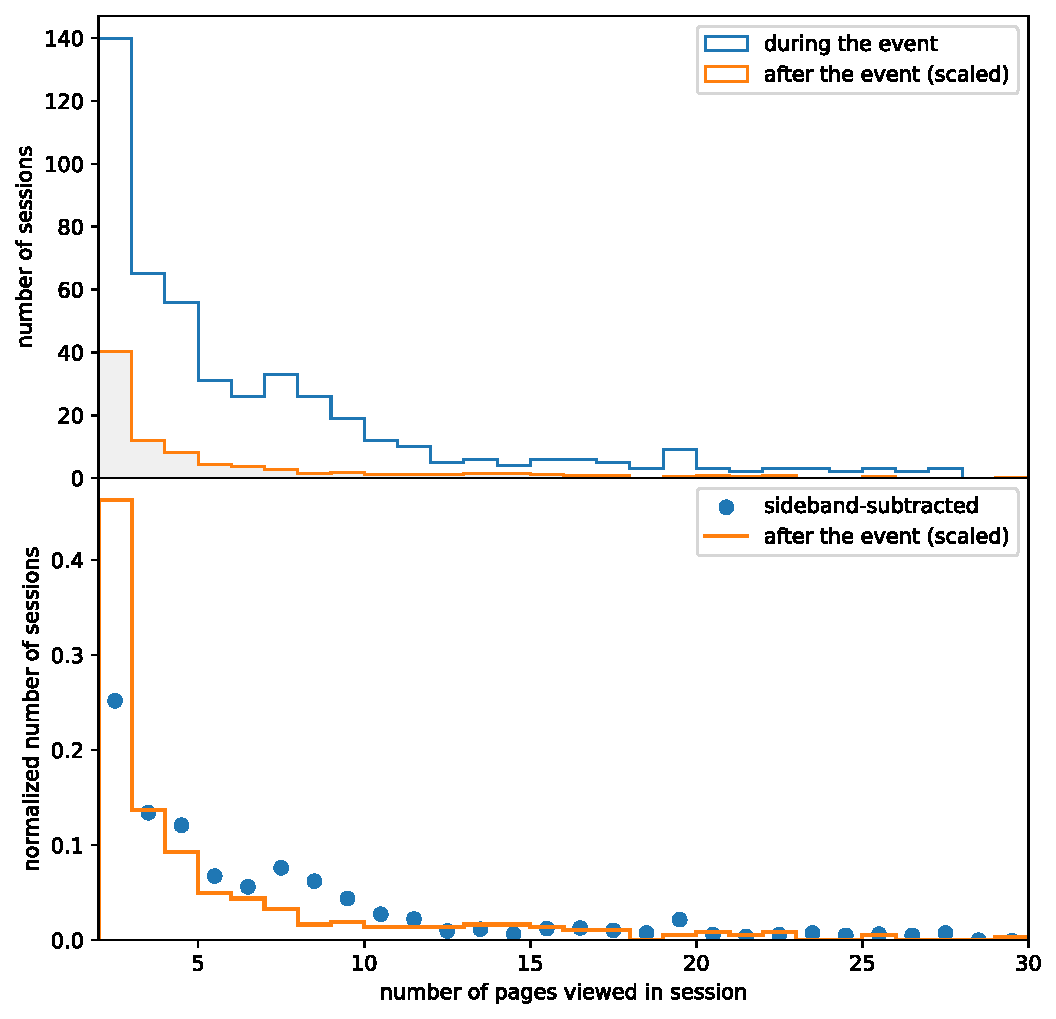
\includegraphics[width=\linewidth]{PLOTS/during-and-after-event-pages-viewed.pdf}
\end{columns}

\vspace{0.75 cm}
\uncover<2->{The distributions look {\it a little} different, but not much different.}

\vspace{0.25 cm}
\uncover<3->{Website visitors weeks after the event are as studious as during.}
\end{frame}

\begin{frame}{(All sources) Breakdown of February 2024 ``Analysis Pipelines''}
\vspace{0.15 cm}
\begin{center}
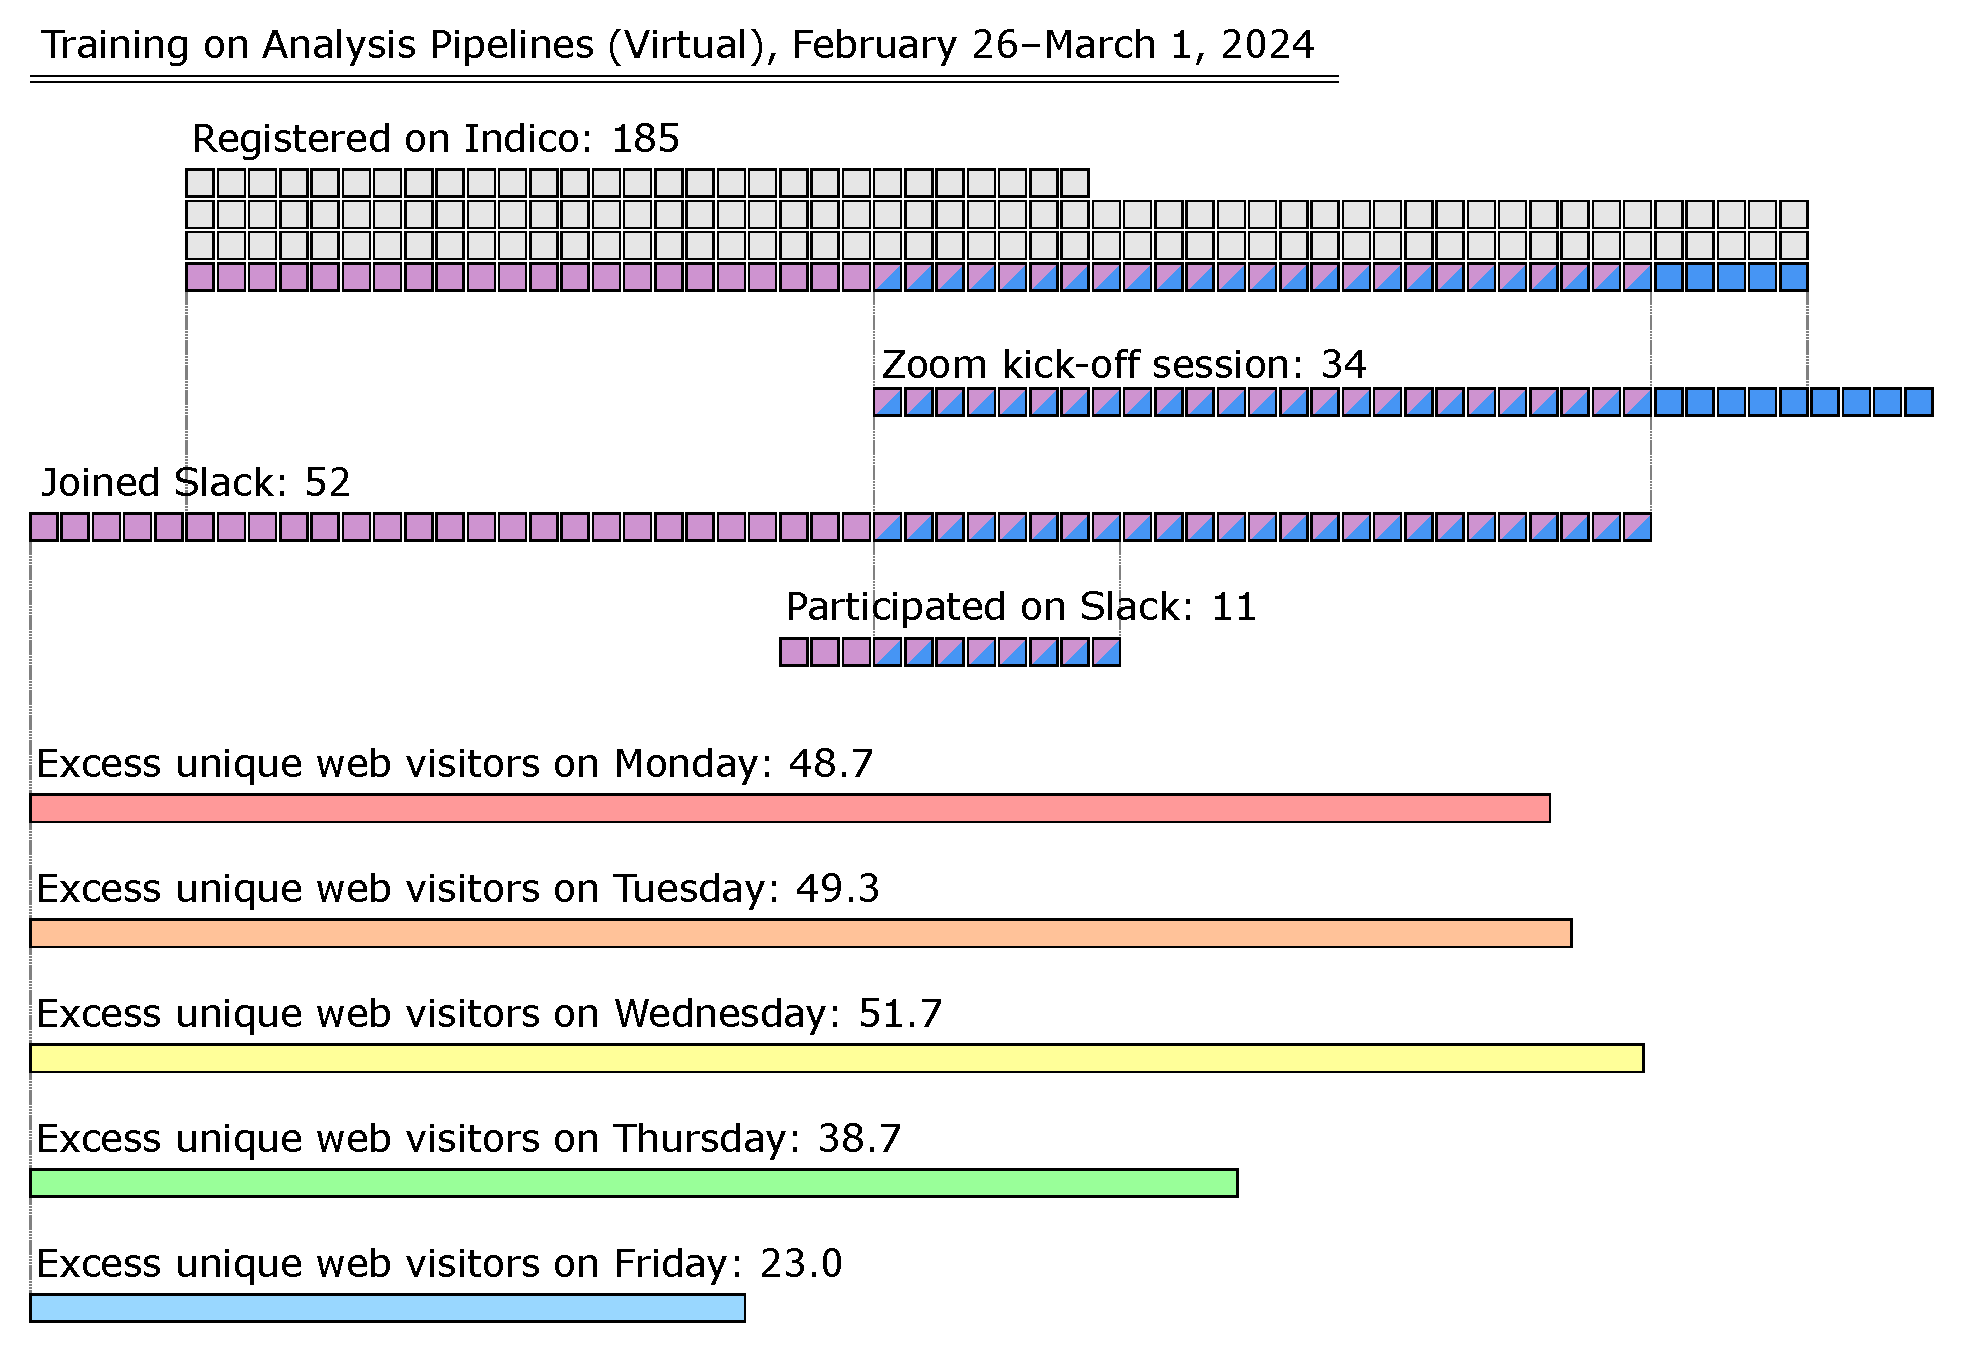
\includegraphics[width=0.8\linewidth]{PLOTS/how-many-participated.pdf}
\end{center}
\end{frame}

\begin{frame}{Conclusions}
\large
\vspace{0.35 cm}
\begin{itemize}\setlength{\itemsep}{0.25 cm}
\item<1-> First conclusion: we have many website visitors who are just as studious as those during an organized training event.

\vspace{0.25 cm}
About 50/day due to the event, but 18.5/day on typical weekdays.

\vspace{0.25 cm}
\begin{itemize}\large
\item<2-> \large Can we make the website more useful for offline studying?
\item<3-> \large Can we scale back the number of organized events per year?
\end{itemize}
\item<4-> The CMake module is especially popular, and we don't even organize a CMake event.
\item<5-> Wildly different distribution of undergrad/grad/postdoc/faculty by event, even events of the same type (not shown in this talk).
\item<6-> There's quite a lot more in the surveys that hasn't been analyzed yet.
\item<7-> How many Spanish-speaking countries in the registrants/website visitors?
\vspace{0.15 cm}
\begin{itemize}\large
\item \large Alex is studying that, to gauge interest in a Spanish translation.
\end{itemize}
\end{itemize}
\end{frame}

\end{document}
